\chapter{Methodology}
\label{chap:methodology}

This chapter provides the methodological foundation for the control policy designed in this thesis. We begin by framing the battery arbitrage problem within the general theory of sequential decision-making, drawing on the unified framework proposed by Powell \cite{powell2022reinforcement}. We then survey the principal families of solution methods that could in principle be applied to this class of problem, justifying our choice of Deep Reinforcement Learning (DRL) over the alternatives. Finally, we present the theoretical underpinnings of the three DRL algorithms that are benchmarked in Chapter~\ref{chap:2}: Deep Q-Network (DQN), Proximal Policy Optimization (PPO), and Soft Actor-Critic (SAC).

% ─────────────────────────────────────────────────────────────────────────────
\section{Sequential Decision-Making}
% ─────────────────────────────────────────────────────────────────────────────

Battery arbitrage in the imbalance market is fundamentally a \textit{sequential decision problem}: at every time step the agent observes a state, chooses an action, receives a reward, and transitions to a new state. The decisions are sequential because each charging or discharging action changes the State of Charge (SoC) and therefore constrains what is possible in all future time steps.

Powell~\cite{powell2022reinforcement} identifies five core components that together define any sequential decision problem:

\begin{enumerate}
    \item \textbf{State} $S_t$: All information available at time $t$ that is needed to make a decision and to model future evolution. In our setting this includes the current SoC and the observed imbalance price signal.
    \item \textbf{Decision / Action} $x_t \in \mathcal{X}$: The control variable chosen by the policy. Here the agent selects one of three discrete actions: charge, discharge, or idle.
    \item \textbf{Exogenous information} $W_{t+1}$: New information that arrives between $t$ and $t+1$ independently of the agent's action—in our case the next imbalance price tick.
    \item \textbf{Transition function} $S^M$: The deterministic or stochastic rule that maps $(S_t, x_t, W_{t+1})$ to $S_{t+1}$. The SoC update and the price process together form this function.
    \item \textbf{Objective function}: The quantity the agent seeks to maximise over the horizon $T$, which in our formulation is the expected cumulative net revenue discounted by $\gamma$.
\end{enumerate}

A policy $\pi$ is any function that maps a state $S_t$ to a decision $x_t$. The objective is to find the policy $\pi^*$ that maximises the expected discounted sum of rewards:
\[
    \pi^* = \arg\max_{\pi}\; \mathbb{E} \left[ \sum_{t=0}^{T} \gamma^t R(S_t,\, \pi(S_t)) \right]
\]

Powell further classifies policies into four broad archetypes: (1) policy function approximations (PFA), (2) cost function approximations (CFA), (3) value function approximations (VFA), and (4) direct lookahead policies (DLA). The heuristic described in Section~\ref{chap:2} is a PFA: a hand-crafted rule that maps state to action. DRL belongs to the VFA and PFA families depending on the specific algorithm. The Oracle is a DLA with perfect lookahead.

% ─────────────────────────────────────────────────────────────────────────────
\section{Solution Method Families}
\label{sec:solution-families}
% ─────────────────────────────────────────────────────────────────────────────

Several families of methods have been applied to energy storage dispatch and imbalance market participation problems. We briefly survey each and explain why DRL is the most suitable choice for the problem at hand.

\subsection{Mathematical Programming}

Linear and mixed-integer programming (MIP) formulate the dispatch problem as an optimisation model with a linear or convex objective and constraints encoding the battery dynamics. Given a perfect price forecast over the horizon $T$, the optimal charging schedule can be found exactly and efficiently \cite{[search: mixed-integer programming battery energy storage arbitrage scheduling]}. However, these methods are \textit{deterministic}: they require a price forecast as input and cannot adapt online to price deviations. In the imbalance market, the settlement price is unknown until the end of each quarter, making a deterministic model systematically vulnerable to forecast errors.

\subsection{Stochastic and Robust Optimisation}

Stochastic programming extends MIP by treating future prices as random variables with a known (or estimated) distribution, optimising over scenarios \cite{[search: stochastic programming electricity storage price uncertainty scenarios]}. Robust optimisation instead seeks a policy that performs well in the worst case over a bounded uncertainty set \cite{[search: robust optimisation battery storage imbalance market energy]}. Both approaches improve on deterministic MIP but at a steep computational cost: the scenario tree grows exponentially with the horizon, and both methods require an explicit probabilistic model of the price process—an assumption that is difficult to justify for the highly non-stationary Belgian imbalance market.

\subsection{Model Predictive Control}

Model Predictive Control (MPC) solves a deterministic or stochastic optimisation problem over a receding horizon at each time step, using the latest price forecast \cite{[search: model predictive control battery energy storage real-time dispatch]}. MPC has been successfully applied to building energy management and grid-scale storage, but its performance is tightly coupled to forecast quality. Furthermore, it must re-solve an optimisation problem at every decision step, imposing a latency constraint that may be impractical for minute-level imbalance decisions.

\subsection{Approximate Dynamic Programming}

Approximate Dynamic Programming (ADP) directly approximates the value function $V(S_t)$ of the Bellman equation using parametric function approximators, iteratively improving the approximation through simulation \cite{powell2022reinforcement}. ADP is well-suited to problems with continuous state spaces and avoids the curse of dimensionality that renders exact DP intractable. Indeed, as shown in Section~\ref{chap:2}, exact backward DP is only feasible for the base model precisely because the SoC can be perfectly discretised into nine states. Extensions that introduce continuous action spaces or non-linear battery degradation immediately invalidate that tabular approach.

\subsection{Deep Reinforcement Learning}
\label{sec:why-drl}

Deep Reinforcement Learning combines the representational power of deep neural networks with the online, model-free learning paradigm of reinforcement learning. It is uniquely suited to the battery arbitrage problem for three reasons:

\begin{enumerate}
    \item \textbf{Model-free operation:} DRL does not require an explicit probabilistic model of the price process. The agent learns directly from interaction with a simulated environment that replays historical market data, allowing it to capture complex, non-linear price dynamics that are difficult to model analytically \cite{li2018deepreinforcementlearningoverview, ZHENG2024112084}.
    \item \textbf{Scalability to richer state spaces:} Because the policy and value functions are represented by neural networks, extending the state space with new features (e.g., time-of-day encodings, rolling price statistics, or weather covariates) requires only a change to the input layer, not a re-derivation of the optimisation model.
    \item \textbf{Adaptability to environment complexity:} As argued in Section~\ref{chap:2}, introducing continuous actions, round-trip efficiency losses, or degradation-dependent cycle costs breaks the tabular DP approach entirely but poses no fundamental obstacle to a DRL agent.
\end{enumerate}

These properties motivate the exclusive use of DRL for the remainder of this thesis. The next section presents the theoretical underpinnings of the three algorithms benchmarked in Chapter~\ref{chap:2}.

% ─────────────────────────────────────────────────────────────────────────────
\section{Deep Reinforcement Learning Algorithms}
\label{sec:drl-algorithms}
% ─────────────────────────────────────────────────────────────────────────────

All DRL algorithms share the same Markov Decision Process (MDP) formulation: an agent observes state $S_t$, selects action $x_t$ according to policy $\pi_\theta$, receives reward $R_{t+1}$, and transitions to $S_{t+1}$. They differ in \textit{how} they represent and update the policy. Table~\ref{tab:algorithm-comparison} summarises the key axes along which the three evaluated algorithms differ.

\begin{table}[h]
    \centering
    \renewcommand{\arraystretch}{1.3}
    \begin{tabular}{l c c c}
        \hline
        \textbf{Property} & \textbf{DQN} & \textbf{PPO} & \textbf{SAC} \\
        \hline
        Policy type        & Value-based (implicit) & Policy gradient (explicit) & Policy gradient (explicit) \\
        On/Off-policy      & Off-policy             & On-policy                  & Off-policy \\
        Exploration        & $\varepsilon$-greedy   & Entropy bonus              & Max-entropy objective \\
        Experience replay  & \checkmark             & $\times$                   & \checkmark \\
        Dual critics       & $\times$               & $\times$                   & \checkmark \\
        \hline
    \end{tabular}
    \caption{Comparison of the three evaluated DRL algorithms along key architectural dimensions.}
    \label{tab:algorithm-comparison}
\end{table}

\subsection{Deep Q-Network (DQN)}
\label{sec:dqn-theory}

DQN \cite{mnih2013playing} is a \textit{value-based} method: it learns the optimal action-value function $Q^*(S_t, A_t)$ and derives the policy implicitly as $\pi(S_t) = \arg\max_a Q(S_t, a;\,\theta)$.

\paragraph{Q-Learning and the Bellman Equation}
The optimal action-value function satisfies the Bellman optimality equation:
\[
    Q^*(S_t, A_t) = \mathbb{E} \left[ R_{t+1} + \gamma \max_{a} Q^*(S_{t+1}, a) \right]
\]
Classical (tabular) Q-learning iteratively refines estimates of $Q$ using Temporal Difference (TD) updates:
\[
    Q(S_t, A_t) \leftarrow Q(S_t, A_t) + \alpha \underbrace{\left[ R_{t+1} + \gamma \max_{a} Q(S_{t+1}, a) - Q(S_t, A_t) \right]}_{\text{TD error}}
\]
where $\alpha$ is the learning rate. The agent balances exploration and exploitation via an $\varepsilon$-greedy policy: with probability $\varepsilon$ it takes a random action; otherwise it selects $\arg\max_a Q(S_t, a)$. The value of $\varepsilon$ decays over training as the Q-table is progressively filled with reliable estimates.

\paragraph{From Tabular Q-Learning to Deep Q-Networks}
Maintaining a discrete Q-table is infeasible when the state space contains continuous variables. DQN replaces the table with a deep neural network parameterised by $\theta$, taking state $S_t$ as input and outputting Q-values for all actions simultaneously. Training minimises the mean-squared TD error via gradient descent. To stabilise learning, DQN employs three mechanisms \cite{mnih2015humanlevel}:

\begin{enumerate}
    \item \textbf{Experience Replay:} Transitions $(S_t, A_t, R_{t+1}, S_{t+1})$ are stored in a replay buffer and sampled in random mini-batches, breaking temporal autocorrelation.
    \item \textbf{Fixed Q-Targets:} A frozen target network $\theta^-$ computes the TD target $R_{t+1} + \gamma \max_{a} Q(S_{t+1}, a;\,\theta^-)$, preventing the optimisation target from shifting at every step. The target weights are periodically synchronised with $\theta$.
    \item \textbf{$\varepsilon$-Greedy Decay:} A scheduled reduction of $\varepsilon$ forces broad exploration early in training and transitions the agent to deterministic exploitation as the Q-network matures.
\end{enumerate}

\begin{figure}[h]
    \centering
    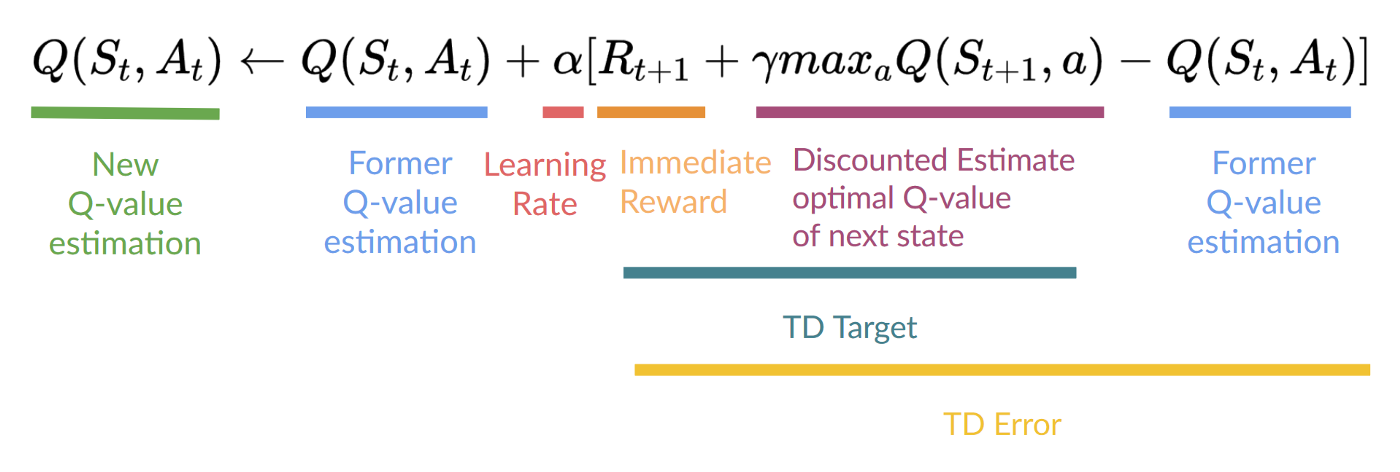
\includegraphics[width=\textwidth]{images/Q-learning-theory/Q-learning-8.jpg}
    \caption{Visual breakdown of the Q-learning state-action value function update equation.}
    \label{fig:q-learning-action-value-update-method}
\end{figure}

\subsection{Proximal Policy Optimization (PPO)}
\label{sec:ppo-theory}

PPO \cite{schulman2017proximal} belongs to the \textit{policy gradient} family: instead of deriving a policy from a value function, it directly parameterises the policy $\pi_\theta$ and optimises it by gradient ascent on expected return.

\paragraph{Policy Gradient Methods}
The objective is to maximise:
\[
    J(\theta) = \mathbb{E}_{\pi_\theta} \left[ \sum_{t=0}^{T} \gamma^t R(S_t, x_t) \right]
\]
The policy gradient theorem states that the gradient of this objective is:
\[
    \nabla_\theta J(\theta) = \mathbb{E}_{\pi_\theta} \left[ \nabla_\theta \log \pi_\theta(x_t \mid S_t) \cdot G_t \right]
\]
where $G_t$ is the return from time $t$. Actions that led to high returns have their log-probabilities increased; actions that led to low returns have theirs decreased.

\paragraph{The Actor-Critic Architecture}
Using the raw return $G_t$ as the learning signal is noisy. PPO adopts an Actor-Critic architecture to reduce variance:
\begin{itemize}
    \item \textbf{Actor ($\pi_\theta$):} Maps state $S_t$ to a probability distribution over actions.
    \item \textbf{Critic ($V_\phi$):} Estimates the expected return from state $S_t$, denoted $\hat{V}(S_t)$.
\end{itemize}
The \textit{Advantage} $\hat{A}_t = G_t - \hat{V}(S_t)$ replaces the raw return in the gradient update, centering the signal around zero and making updates far less sensitive to the scale of absolute rewards.

\paragraph{The Clipped Surrogate Objective}
A fundamental instability in policy gradient training is that a too-large gradient step can collapse the policy irreversibly. PPO prevents this by clipping the probability ratio $r_t(\theta) = \pi_\theta(x_t \mid S_t) / \pi_{\theta_\text{old}}(x_t \mid S_t)$ within the interval $[1-\varepsilon,\, 1+\varepsilon]$:
\[
    \mathcal{L}^{\text{CLIP}}(\theta) = \mathbb{E}_t \left[ \min \left( r_t(\theta)\,\hat{A}_t,\; \text{clip}(r_t(\theta),\, 1-\varepsilon,\, 1+\varepsilon)\,\hat{A}_t \right) \right]
\]
If an update would move the policy too far from the data-collection policy, the gradient is zeroed out at the clip boundary. The result is a ``little-but-often'' learning schedule of safe, monotonically improving updates.

\begin{figure}[h]
    \centering
    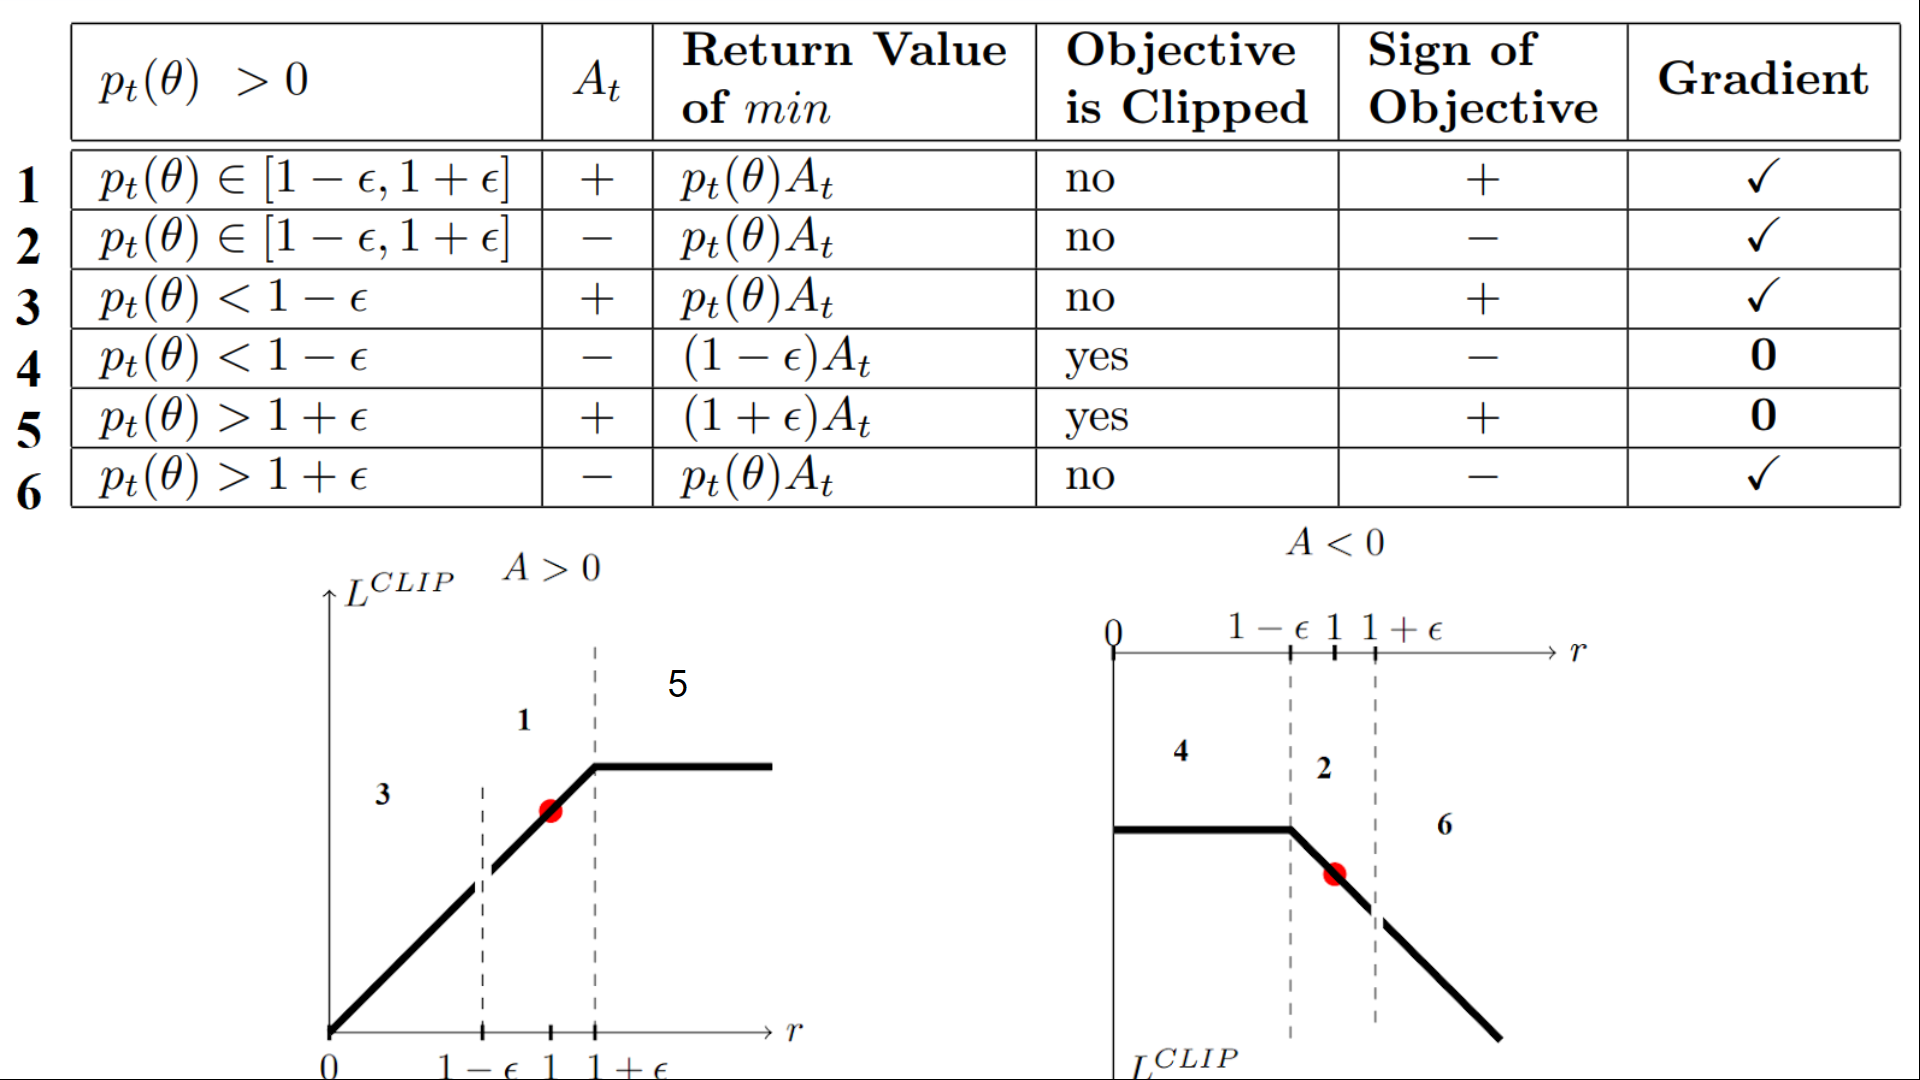
\includegraphics[width=\textwidth]{images/Q-learning-theory/table-ppo.png}
    \caption{Visual breakdown of the clipping procedure in PPO.}
    \label{fig:ppo-clipping-method}
\end{figure}

\paragraph{On-Policy Collection and Entropy Regularisation}
PPO is an \textit{on-policy} algorithm: it collects a fresh batch of transitions with the current policy, performs several gradient epochs, and discards the data. An entropy bonus $\mathcal{H}[\pi_\theta(\cdot \mid S_t)]$ is added to the objective to maintain sufficient exploration and prevent premature commitment to a suboptimal strategy.

\subsection{Soft Actor-Critic (SAC)}
\label{sec:sac-theory}

SAC \cite{haarnoja2018soft} combines the off-policy sample efficiency of DQN with the actor-critic structure of PPO, and adds a distinctive maximum-entropy learning objective.

\paragraph{The Maximum Entropy Framework}
SAC augments the standard RL objective with an entropy bonus at every time step:
\[
    J_{\text{SAC}}(\theta) = \mathbb{E}_{\pi_\theta} \left[ \sum_{t=0}^{T} \gamma^t \Bigl( R(S_t, x_t) + \alpha \,\mathcal{H}\bigl[\pi_\theta(\cdot \mid S_t)\bigr] \Bigr) \right]
\]
where $\alpha > 0$ is the \textit{temperature} parameter. The agent is explicitly rewarded for remaining uncertain, which prevents premature convergence to locally profitable but globally suboptimal strategies—a particular risk in non-stationary markets.

\paragraph{Soft Bellman Equations and Dual Q-Networks}
The entropy-augmented objective induces a revised Bellman equation. The soft value function integrates both expected Q-value and policy entropy:
\[
    V_{\text{soft}}(S_t) = \mathbb{E}_{x_t \sim \pi_\theta} \Bigl[ Q_{\text{soft}}(S_t, x_t) - \alpha \log \pi_\theta(x_t \mid S_t) \Bigr]
\]
SAC maintains \textbf{two independent critic networks} $Q_{\phi_1}$ and $Q_{\phi_2}$. The TD target uses their minimum:
\[
    y = R_{t+1} + \gamma \Bigl( \min_{i=1,2} Q_{\phi_i}(S_{t+1}, x_{t+1}) - \alpha \log \pi_\theta(x_{t+1} \mid S_{t+1}) \Bigr)
\]
This \textit{clipped double-Q} trick counteracts the overestimation bias that would otherwise drive greedy, unstable policies.

\paragraph{Automatic Entropy Tuning}
Rather than treating $\alpha$ as a fixed hyperparameter, SAC solves for the temperature that maintains a target minimum entropy $\bar{\mathcal{H}}$:
\[
    \alpha^* = \arg\min_\alpha\; \mathbb{E}_{x_t \sim \pi_{\theta^*}} \Bigl[ -\alpha \log \pi_{\theta^*}(x_t \mid S_t) - \alpha \bar{\mathcal{H}} \Bigr]
\]
If the policy becomes too deterministic, $\alpha$ increases to encourage exploration; once a reliable strategy is found and entropy already exceeds the target, $\alpha$ decreases to allow confident exploitation. This self-regulating mechanism removes the need for manual temperature tuning across cross-validation folds with different market volatility profiles.

\paragraph{Off-Policy Data Collection}
Like DQN, SAC stores transitions in a replay buffer and draws random mini-batches for every gradient update. This off-policy mechanism decouples data collection from learning, making SAC substantially more \textit{sample efficient} than the on-policy PPO: every market transition can contribute to many gradient updates, amortising the cost of environmental interaction.
